\section{Модальный регулятор}

Рассматриваем систему
\begin{equation}
    \dot x = Ax+Bu,\quad
    A=\begin{bmatrix}
        3 & 5 & 4 \\
        -2 & -4 & -5 \\
        2 & 2 & 3
    \end{bmatrix},\quad
    B=\begin{bmatrix}
        2 \\ -1 \\ 1
    \end{bmatrix}.
    \label{eq:1}
\end{equation}
Спектр матрицы $A$
\begin{equation*}
    \sigma(A)=\{2\pm i,\ -2\}.
\end{equation*}
Построив матрицы Хаутуса, делаем вывод, что сопряженная пара
собственных чисел управляема, а вещественное число $-2$ - нет,
но так как оно отрицательное, то система стабилизируема, хотя и
не полностю управляема. 

\subsection{Синтез модального регулятора}

Построим структурную схему системы \autoref{fig:1} 
с замкнутым регулятором вида $u=Kx$.
\begin{figure}[H]
    \centering
    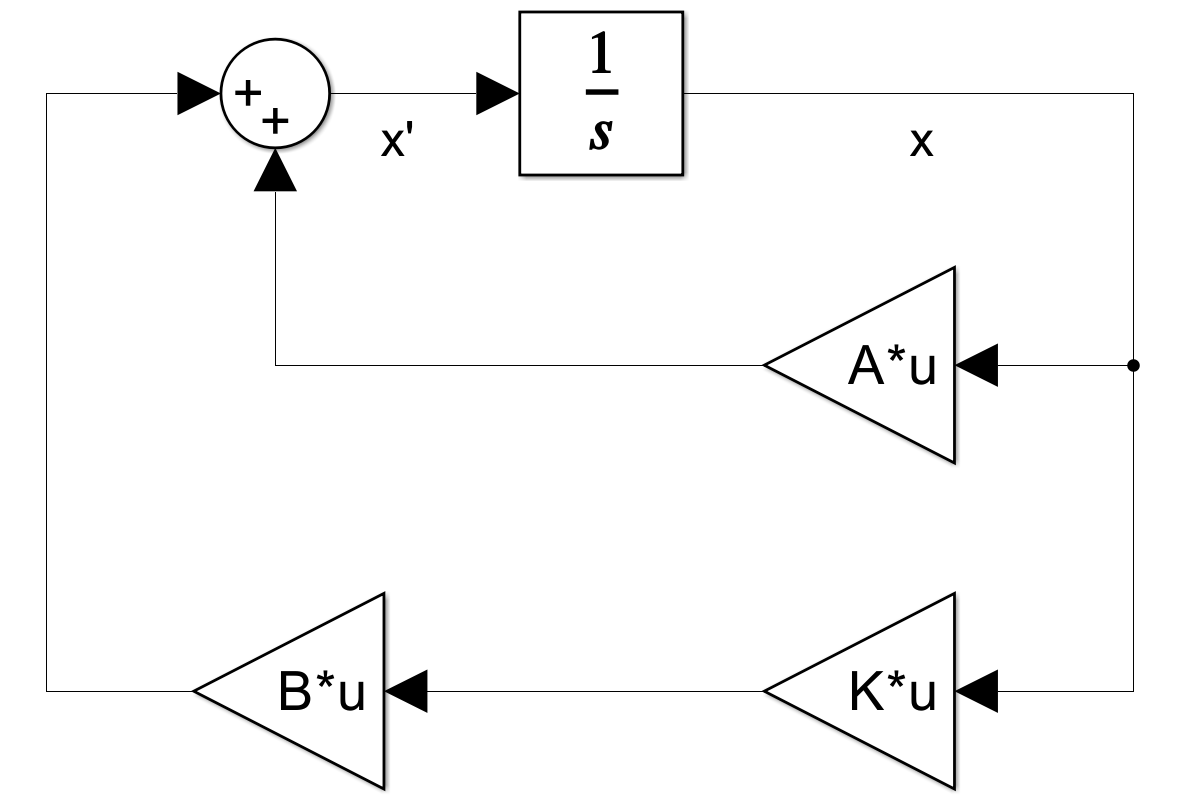
\includegraphics[width=0.7\linewidth]{figs/task1_slx.png}
    \caption{Схема моделирования системы \ref{eq:1}, замкнутой
    регулятором вида $u=Kx$}
    \label{fig:1}
\end{figure}
\noindent Для синтеза модального регулятора предложены 
данные варианты спектра $\sigma(A+BK)$:
\begin{equation*}
    \begin{array}{rl}
        \{-1,\ -1,\ -1\}, & \{-2,\ -2,\ -2\}, \\
        \{-1,\ -10,\ -100\}, & \{-2,\ -20,\ -200\}, \\
        \{-1,\ -1\pm 3i\}, & \{-2,\ -2\pm 6i\}.
    \end{array}
\end{equation*}
Спектры, которые не содержат $-2$ недостежимы, так как
данное собственное число неуправляемо, оно всегда будет
присутствовать в спектре системы. Оставшиеся
3 спектра достежимы.

\subsubsection{Первый спектр}

Получим спектр $\{-2,\ -2,\ -2\}$. Так как одно из собственных чисел неуправляемо систему
придется "усечь" для синтеза модального регулятора.
Жорданова форма системы выглядит следующим образом
\begin{equation*}
    \dot{\hat x} = A_J\hat x+B_Ju,\quad A_J=\begin{bmatrix}
        -2&     0 &    0\\
        0  &   2 &   -1\\
        0   &  1&     2
    \end{bmatrix},\quad
    B_J=\begin{bmatrix}
        0\\
        0.7071\\
       -2.1213
    \end{bmatrix}.
\end{equation*}
Вычеркнем элементы, соответствующие неуправляемым 
собственным числам, получив
\begin{equation*}
    A_J^*=\begin{bmatrix}
        2 & -1 \\ 1 & 2
    \end{bmatrix},\quad
    B_J^*=\begin{bmatrix}
        0.7071\\
       -2.1213
    \end{bmatrix}.
\end{equation*}
Находим $K_J^*$ с помощью решения уравнения Сильвестра относительно матрицы $P$:
\begin{equation*}
    A_J^*P-P\Gamma = B_J^*Y,
\end{equation*}
где $\Gamma$ - матрица, имеющая интересующий нас спектр, а $Y$ подобрана так, чтобы
пара $(\Gamma, Y)$ была наблюдаема. Решение находим с помощью CVX и далее получаем
желаемую матрицу:
\begin{equation*}
    K_J^*=-YP^{-1}=\begin{bmatrix}
        -7.4954&     1.2728
    \end{bmatrix},
\end{equation*}
дополним нулем
\begin{equation*}
    K_J=\begin{bmatrix}
        0 & -7.4954&     1.2728
    \end{bmatrix}.
\end{equation*}

\noindent Найдем $K_J$ в исходном бызисе
системы, а не в жордановом ($P$ - матрица перехода)
\begin{equation*}
    K=K_JP^{-1}=\begin{bmatrix}
        -1.8000	&-1.8000	&-6.2001
    \end{bmatrix}
\end{equation*}

\begin{figure}[H]
    \centering
    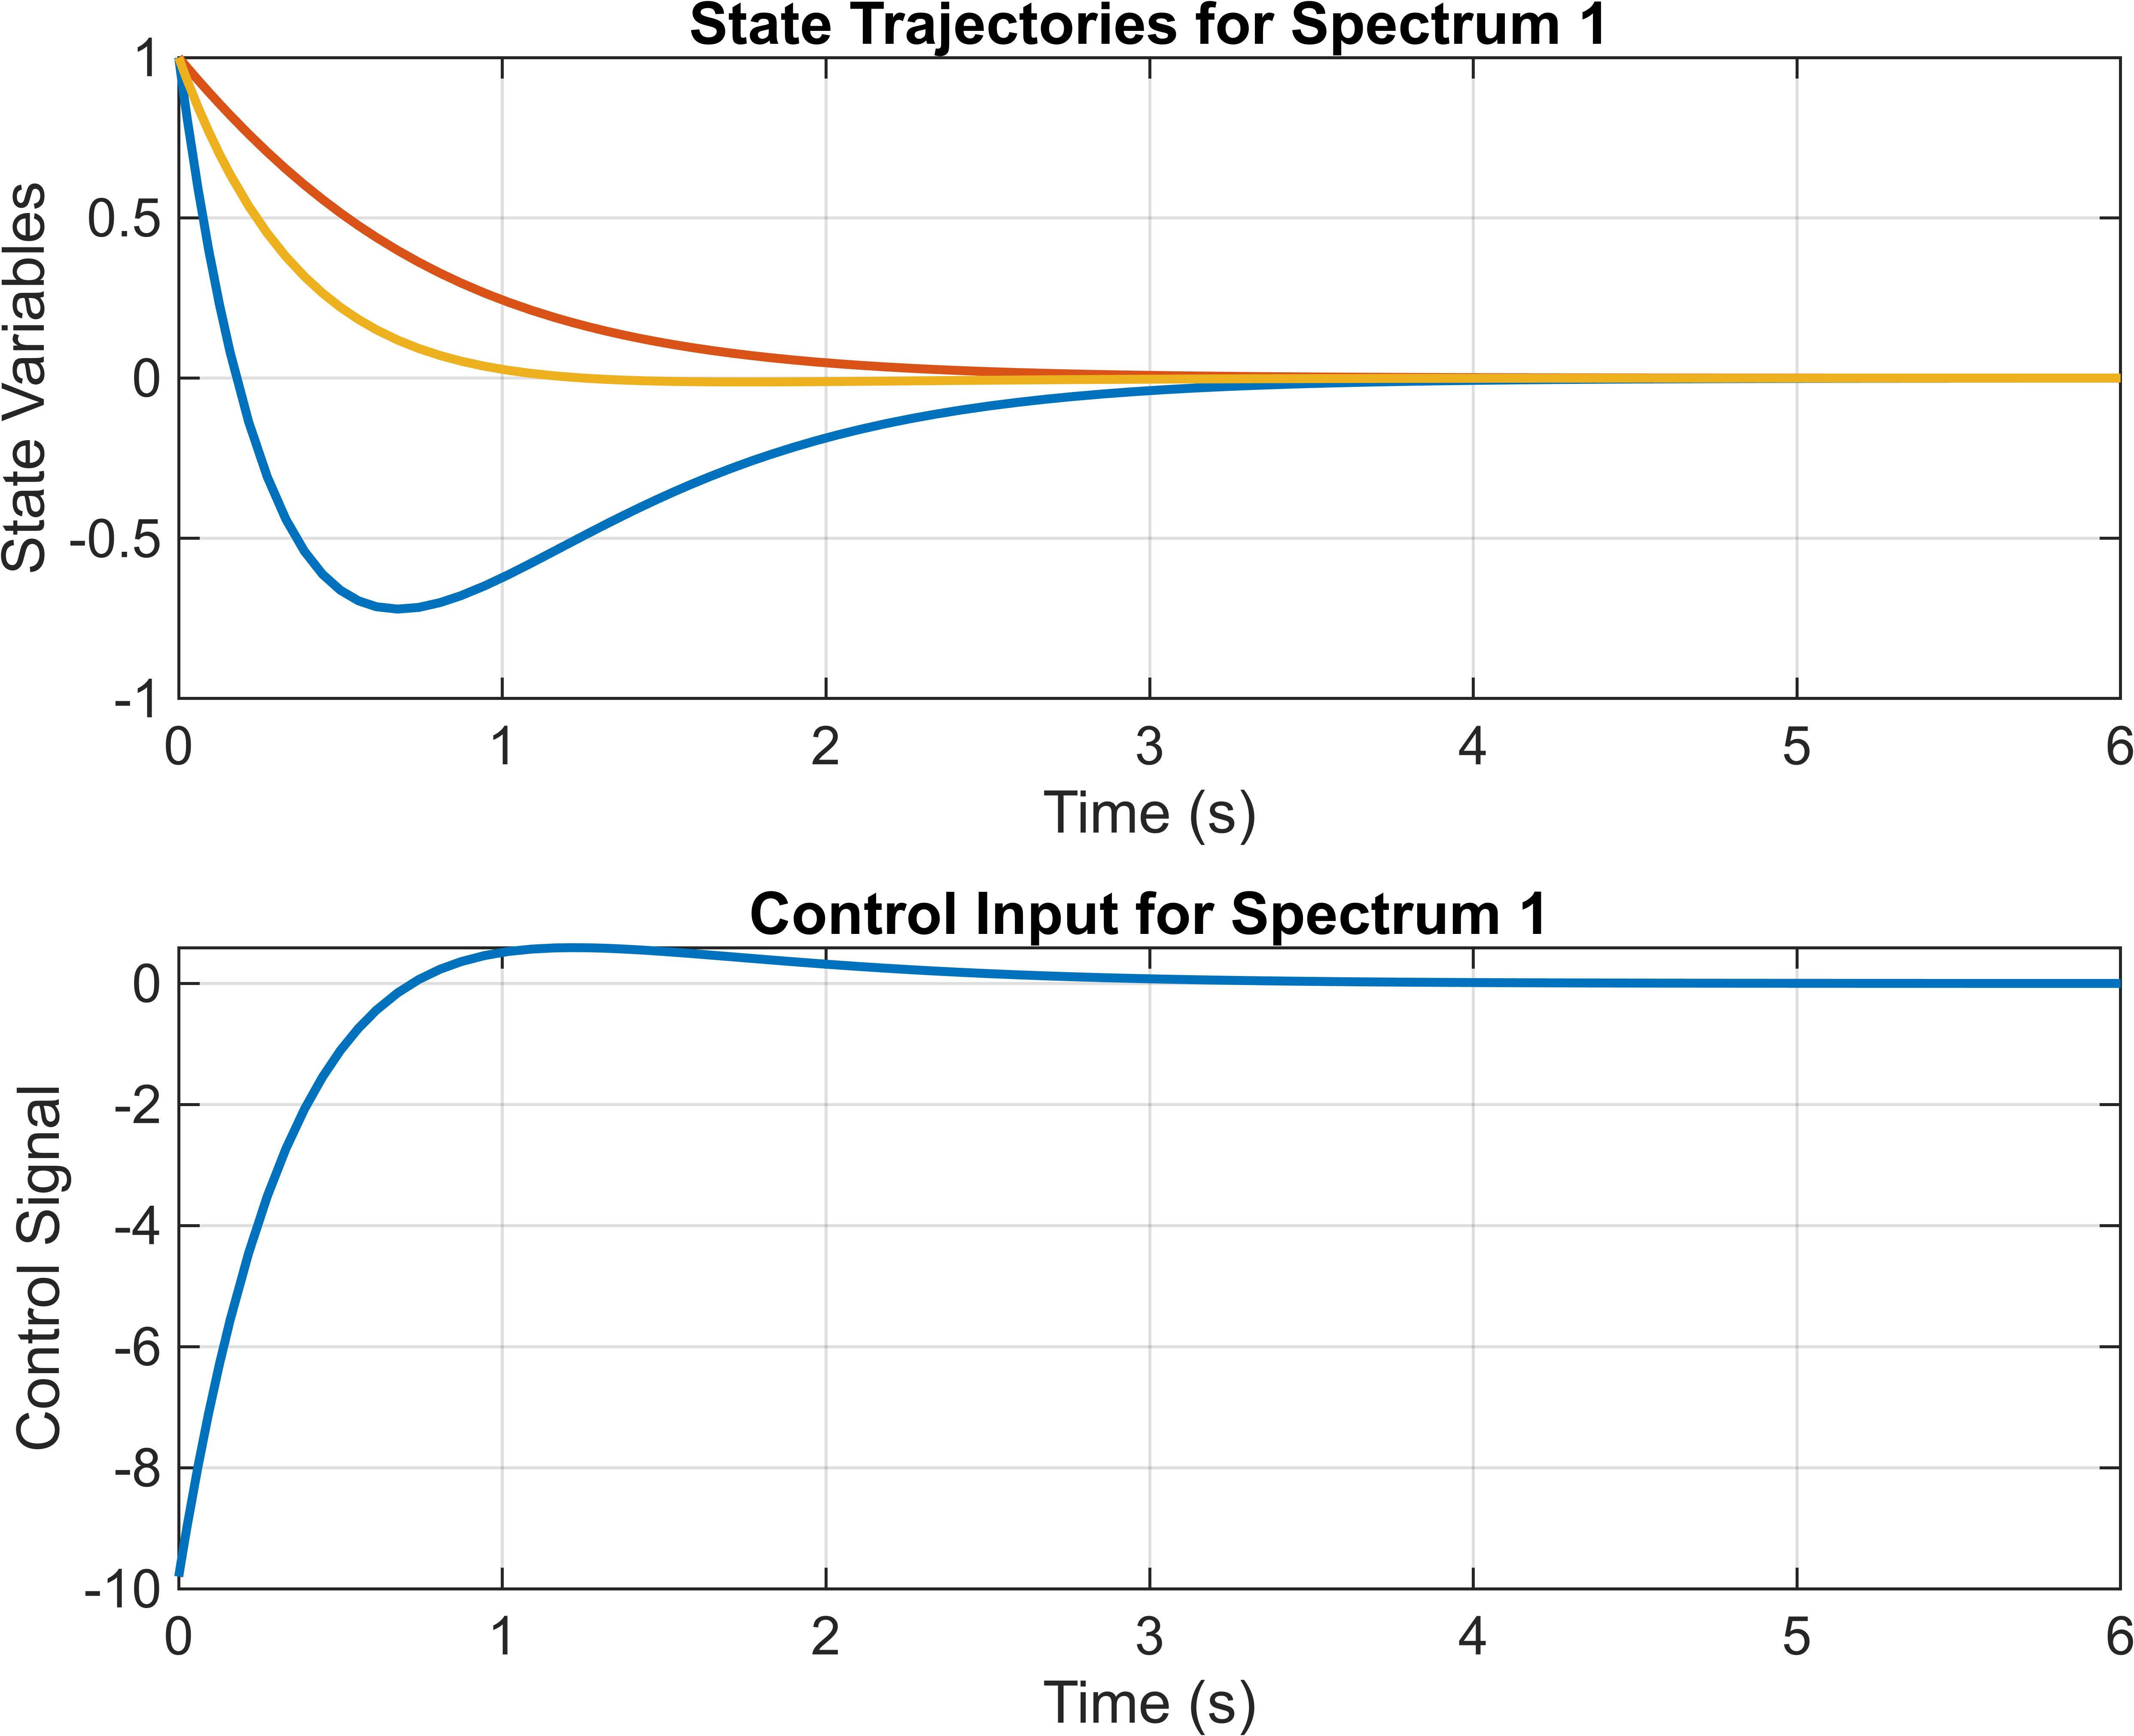
\includegraphics[width=0.9\linewidth]{figs/task1_1.png}
    \caption{Управление и состояние системы с модальным регулятором для первого спектра}
    \label{fig:1_1}
\end{figure}

\noindent и проверим результат
\begin{equation*}
    \sigma(A+BK)=\{-1.9873,\ 
    -2.0128,\ 
    -2.0000\},
\end{equation*}
заданный спектр успешно получен с небольшой погрешностью. 
Выполним компьютерное моделирование и построим графики 
формируемого регулятором управления $u(t)$ и вектора 
состояния замкнутой системы $x(t)$ при начальном условии 
$x(0) =\begin{bmatrix}
    1 & 1 & 1
\end{bmatrix}^T$, что можно увидеть на \autoref{fig:1_1}.

\subsubsection{Второй спектр}

Получим спектр $\{-2,\ -20,\ -200\}$. Аналогично находим $K_J^*$ с помощью CVX
\begin{equation*}
    K_J^*=\begin{bmatrix}
        -1916.7&	-533.3050
    \end{bmatrix}.
\end{equation*}
Найдем $K_J$ в исходном бызисе
системы, а не в жордановом
\begin{equation*}
    K=\begin{bmatrix}
        754.2072&	754.2072&	-978.2094
    \end{bmatrix}
\end{equation*}
и проверим результат
\begin{equation*}
    \sigma(A+BK)=\{-200.0022,\ 
    -20.0000,\ 
    -2.0000\},
\end{equation*}
заданный спектр успешно получен с небольшой погрешностью. 
Выполним компьютерное моделирование и построим графики 
формируемого управления $u(t)$ и вектора 
состояния $x(t)$ при начальном условии 
$x(0) =\begin{bmatrix}
    1 & 1 & 1
\end{bmatrix}^T$, что можно увидеть на \autoref{fig:1_2}.

\begin{figure}[H]
    \centering
    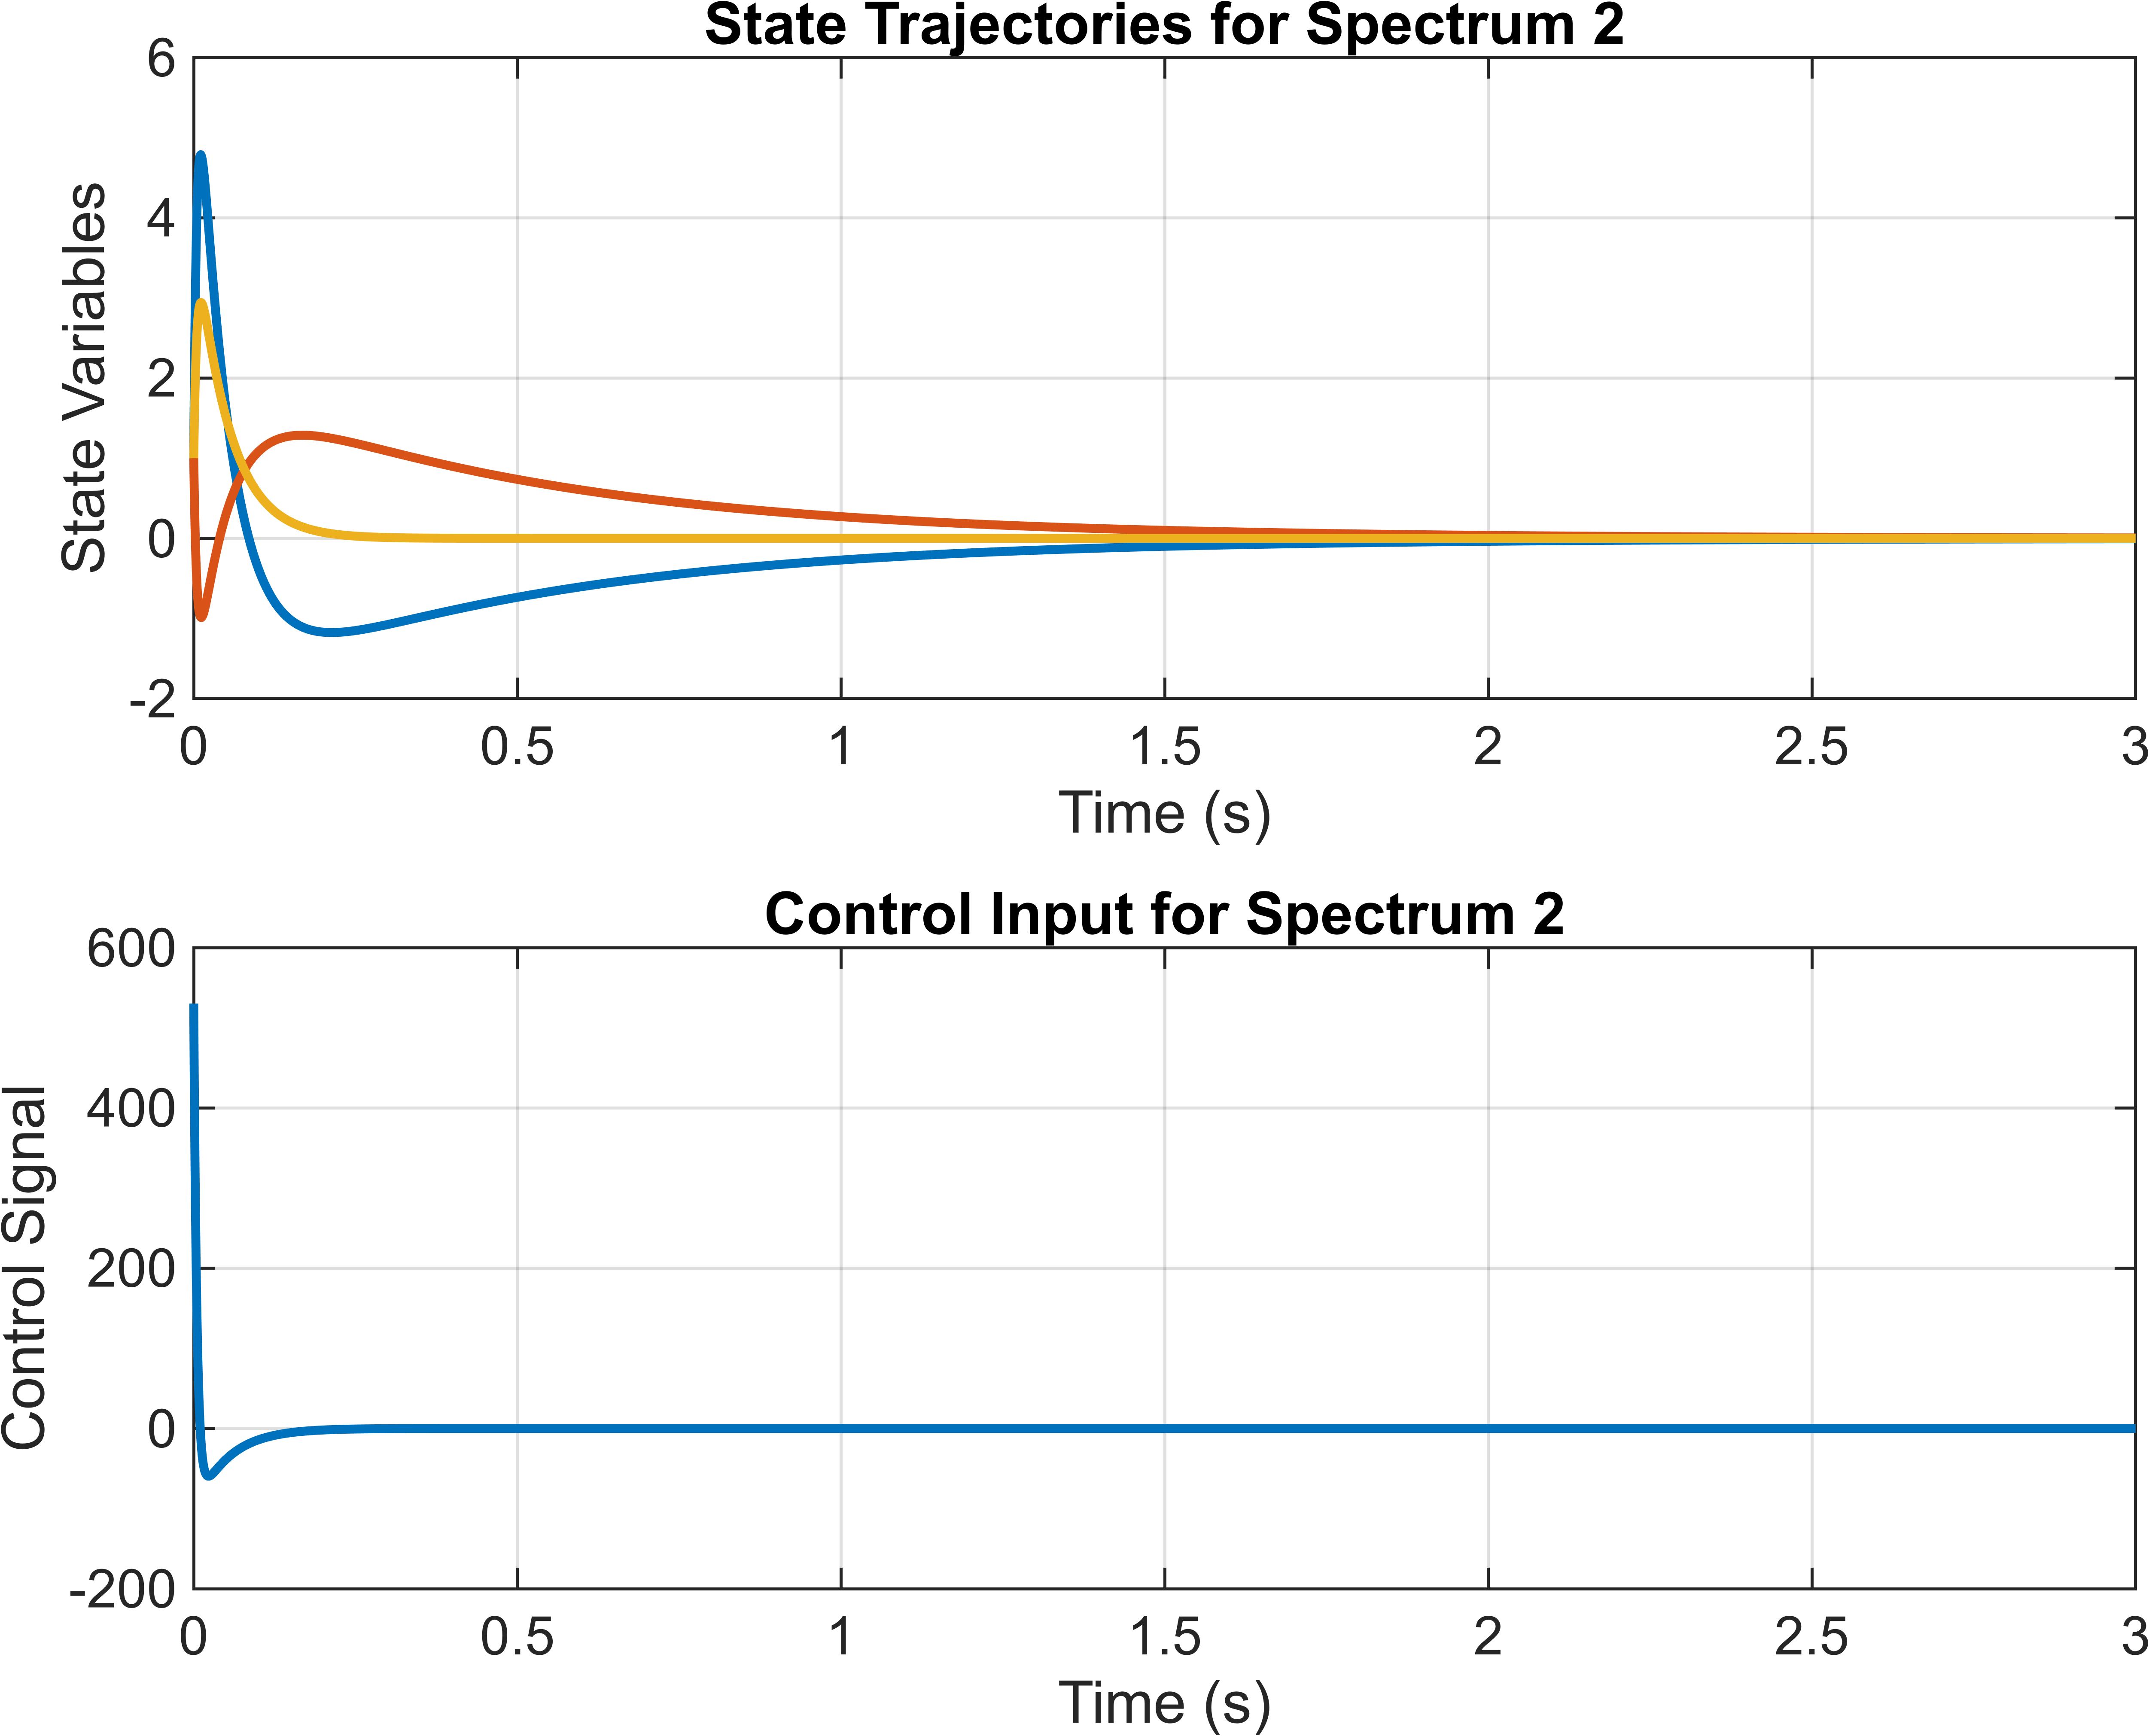
\includegraphics[width=0.9\linewidth]{figs/task1_2.png}
    \caption{Управление и состояние системы с модальным регулятором для второго спектра}
    \label{fig:1_2}
\end{figure}

\subsubsection{Третий спектр}

Получим спектр $\{-2,\ -2\pm 6i\}$. Аналогично находим $K_J^*$ с помощью CVX
\begin{equation*}
    K_J^*=\begin{bmatrix}
        -22.7691&	-3.8184
    \end{bmatrix}.
\end{equation*}
Найдем $K_J$ в исходном бызисе
системы
\begin{equation*}
    K=\begin{bmatrix}
        5.4001&	5.4001&	-13.4001
    \end{bmatrix}
\end{equation*}
и проверим результат
\begin{equation*}
    \sigma(A+BK)=\{-2.0000 + 6.0000i,\ 
    -2.0000 - 6.0000i,\ 
    -2.0000\},
\end{equation*}
заданный спектр успешно получен с точностью до четырех знаков. 
Выполним компьютерное моделирование и построим графики 
формируемого управления $u(t)$ и вектора 
состояния $x(t)$ при начальном условии 
$x(0) =\begin{bmatrix}
    1 & 1 & 1
\end{bmatrix}^T$, что можно увидеть на \autoref{fig:1_3}.

\begin{figure}[H]
    \centering
    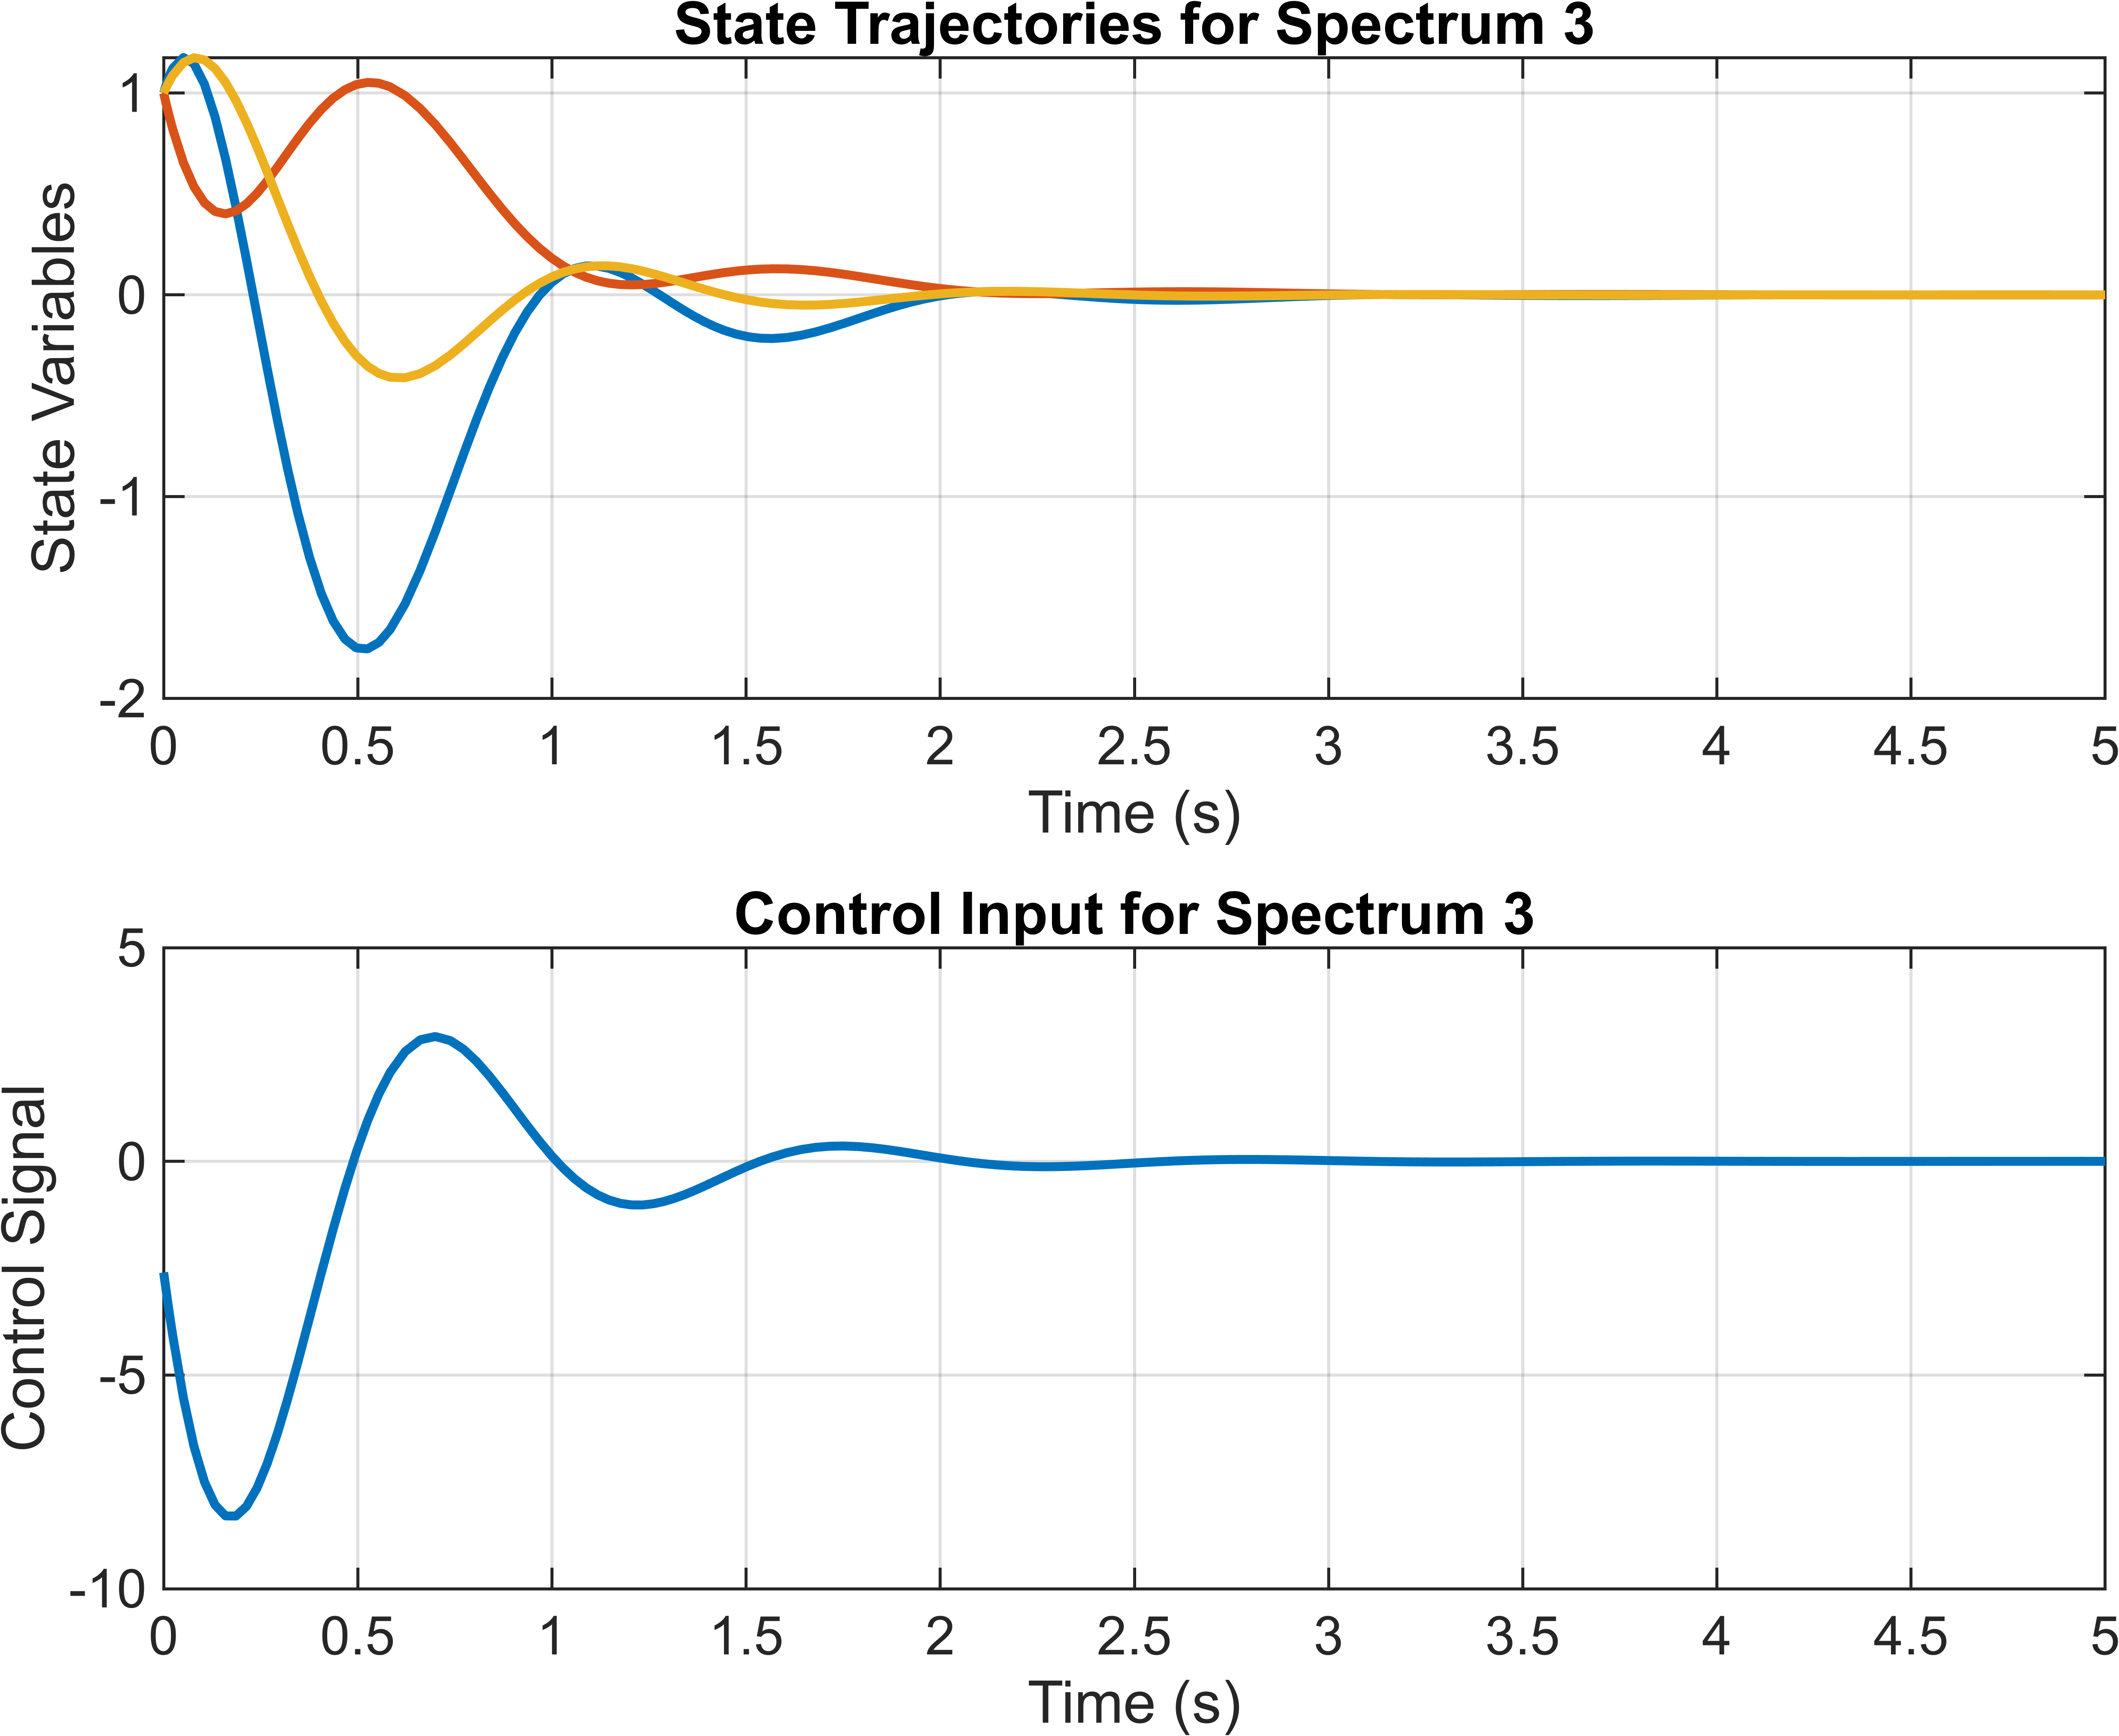
\includegraphics[width=0.9\linewidth]{figs/task1_3.png}
    \caption{Управление и состояние системы с модальным регулятором для третьего спектра}
    \label{fig:1_3}
\end{figure}

\subsection{Вывод}

Сопоставим результаты компьютерного моделирования для рассмотренных спектров.
Для первого спектра $\{-2,\ -2,\ -2\}$:
\begin{itemize}
    \item Система стабилизируется примерно за 5 секунды.
    \item Управление $u(t)$ имеет минимальное значение -10 и максимальное меньше 1.
    \item Вектор состояния $x(t)$ плавно стремится к нулю.
\end{itemize}
Для второго спектра $\{-2,\ -20,\ -200\}$:
\begin{itemize}
    \item Система стабилизируется примерно за 2.5 секунды.
    \item Управление $u(t)$ имеет минимальное значение около -50 и максимальное около 500.
    \item Вектор состояния $x(t)$ очень резко стремится к нулю.
\end{itemize}
Для третьего спектра $\{-2,\ -2\pm 6i\}$:
\begin{itemize}
    \item Система стабилизируется примерно за 3.5 секунды.
    \item Управление $u(t)$ имеет значение от -8 до 3.
    \item Вектор состояния $x(t)$ демонстрирует колебательное поведение перед стабилизацией.
\end{itemize}
Сравнительные преимущества и недостатки:
\begin{itemize}
    \item Первый спектр обеспечивает плавную стабилизацию и управление 
    с умеренными значениями, что делает его подходящим для систем, где требуется
    плавность, так же система не требовательна к величине управления.
    \item Второй спектр обеспечивает самую быструю стабилизацию, но требует очень 
    больших значений управления, что может быть непрактично в реальных системах.
    \item Третий спектр обеспечивает быструю стабилизацию с колебательным поведением, 
    по сравнению с первым спектром мы обменивает плавность движения на скорость стабилизации.
\end{itemize}



\section{Наблюдатель полного порядка}

Рассматриваем систему
\begin{equation}
    \begin{cases}
        \dot x = Ax,\\
        y = Cx,
    \end{cases}\quad
    A=\begin{bmatrix}
        25& 8& -20& 13\\
        -38& -11& 30& -18\\
        40& 13& -33& 21\\
        38& 12& -32& 19
    \end{bmatrix},\quad
    C=\begin{bmatrix}
        7&2&-5&3
    \end{bmatrix}.
    \label{eq:2}
\end{equation}
Спектр матрицы $\sigma(A)= \{\pm3i,\ \pm i\}.$ Построив матрицы Хаутуса, 
делаем вывод, что все собственные числа наблюдаемы. Следовательно
система полностью наблюдаема, а тогда и обнаруживаема.
Построим структурную схему системы \ref{eq:2} c наблюдателем состояния
$\dot{\hat x}=A\hat x+L(C\hat x - y),$ которую можно увидеть на \autoref{fig:2}.

\begin{figure}[H]
    \centering
    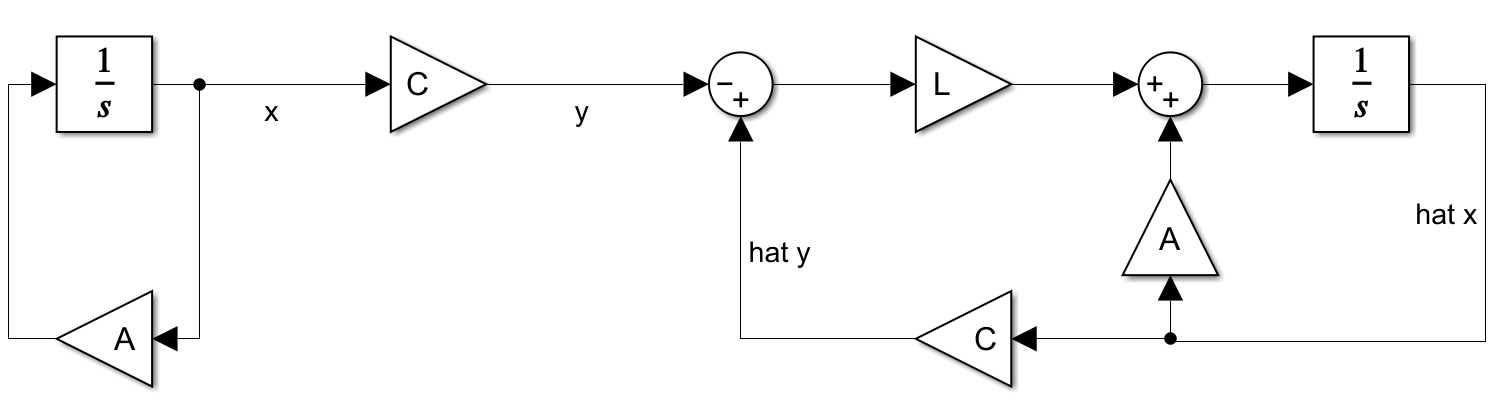
\includegraphics[width=\linewidth]{figs/task2_slx.png}
    \caption{Схема моделирования системы \ref{eq:2} с наблюдателем}
    \label{fig:2}
\end{figure}

\subsection{Синтез наблюдателя}

Варианты спектра $\sigma(A+LC)$
\begin{equation*}
    \begin{array}{c}
        \{-1, -1, -1, -1\}\\
        \{-1, -10, -100, -1000\}\\
        \{-1 \pm 2i, -1 \pm 3i\}
    \end{array}
\end{equation*}


\subsubsection{Первый спектр}

Чтобы получить спектр $\{-1, -1, -1, -1\}$, нужно найти решение уравнения Сильвестра
относительно $Q$
\begin{equation*}
    \Gamma Q-QA=YC,
\end{equation*}
где $\Gamma$ - матрица, имеющая интересующий нас спектр, а $Y$ подобрана так, чтобы
пара $(\Gamma, Y)$ была управляема. Были выбраны такие матрицы
\begin{equation*}
    \Gamma=\begin{bmatrix}
        -1&  1&  0&  0\\
        0& -1&  1&  0\\
        0&  0& -1&  1\\
        0&  0&  0& -1
    \end{bmatrix},\quad
    Y=\begin{bmatrix}
        0\\ 0\\ 0\\ 1
    \end{bmatrix}.
\end{equation*}
Решение находим с помощью CVX и далее получаем
\begin{equation*}
    L=\begin{bmatrix}
        -5.1667\\
5.6667\\
-8.6667\\
-7.5000
    \end{bmatrix}.
\end{equation*}
Проверим, что получен желаемый спектр
\begin{equation*}
    \sigma(A+LC)=\{-1.0005\pm 0.0005i,\ -0.9995\pm 0.0005i\}.
\end{equation*}
Желаемый спектр успешно получен с небольшой погрешностью.
Выполним моделирование с начальными условиями системы 
$x(0) = \begin{bmatrix}
    1 & 1 & 1 & 1
\end{bmatrix}^T$ и наблюдателя $\hat x(0) = \begin{bmatrix}
    2 & 0 & 0 & -1
\end{bmatrix}^T$. Cравнительные графики $x(t)$ и $\hat x(t)$, 
а также график ошибки наблюдателя $e(t) = x(t) -\hat x(t)$
можно увидеть на \autoref{fig:2_1}.

\begin{figure}[H]
    \centering
    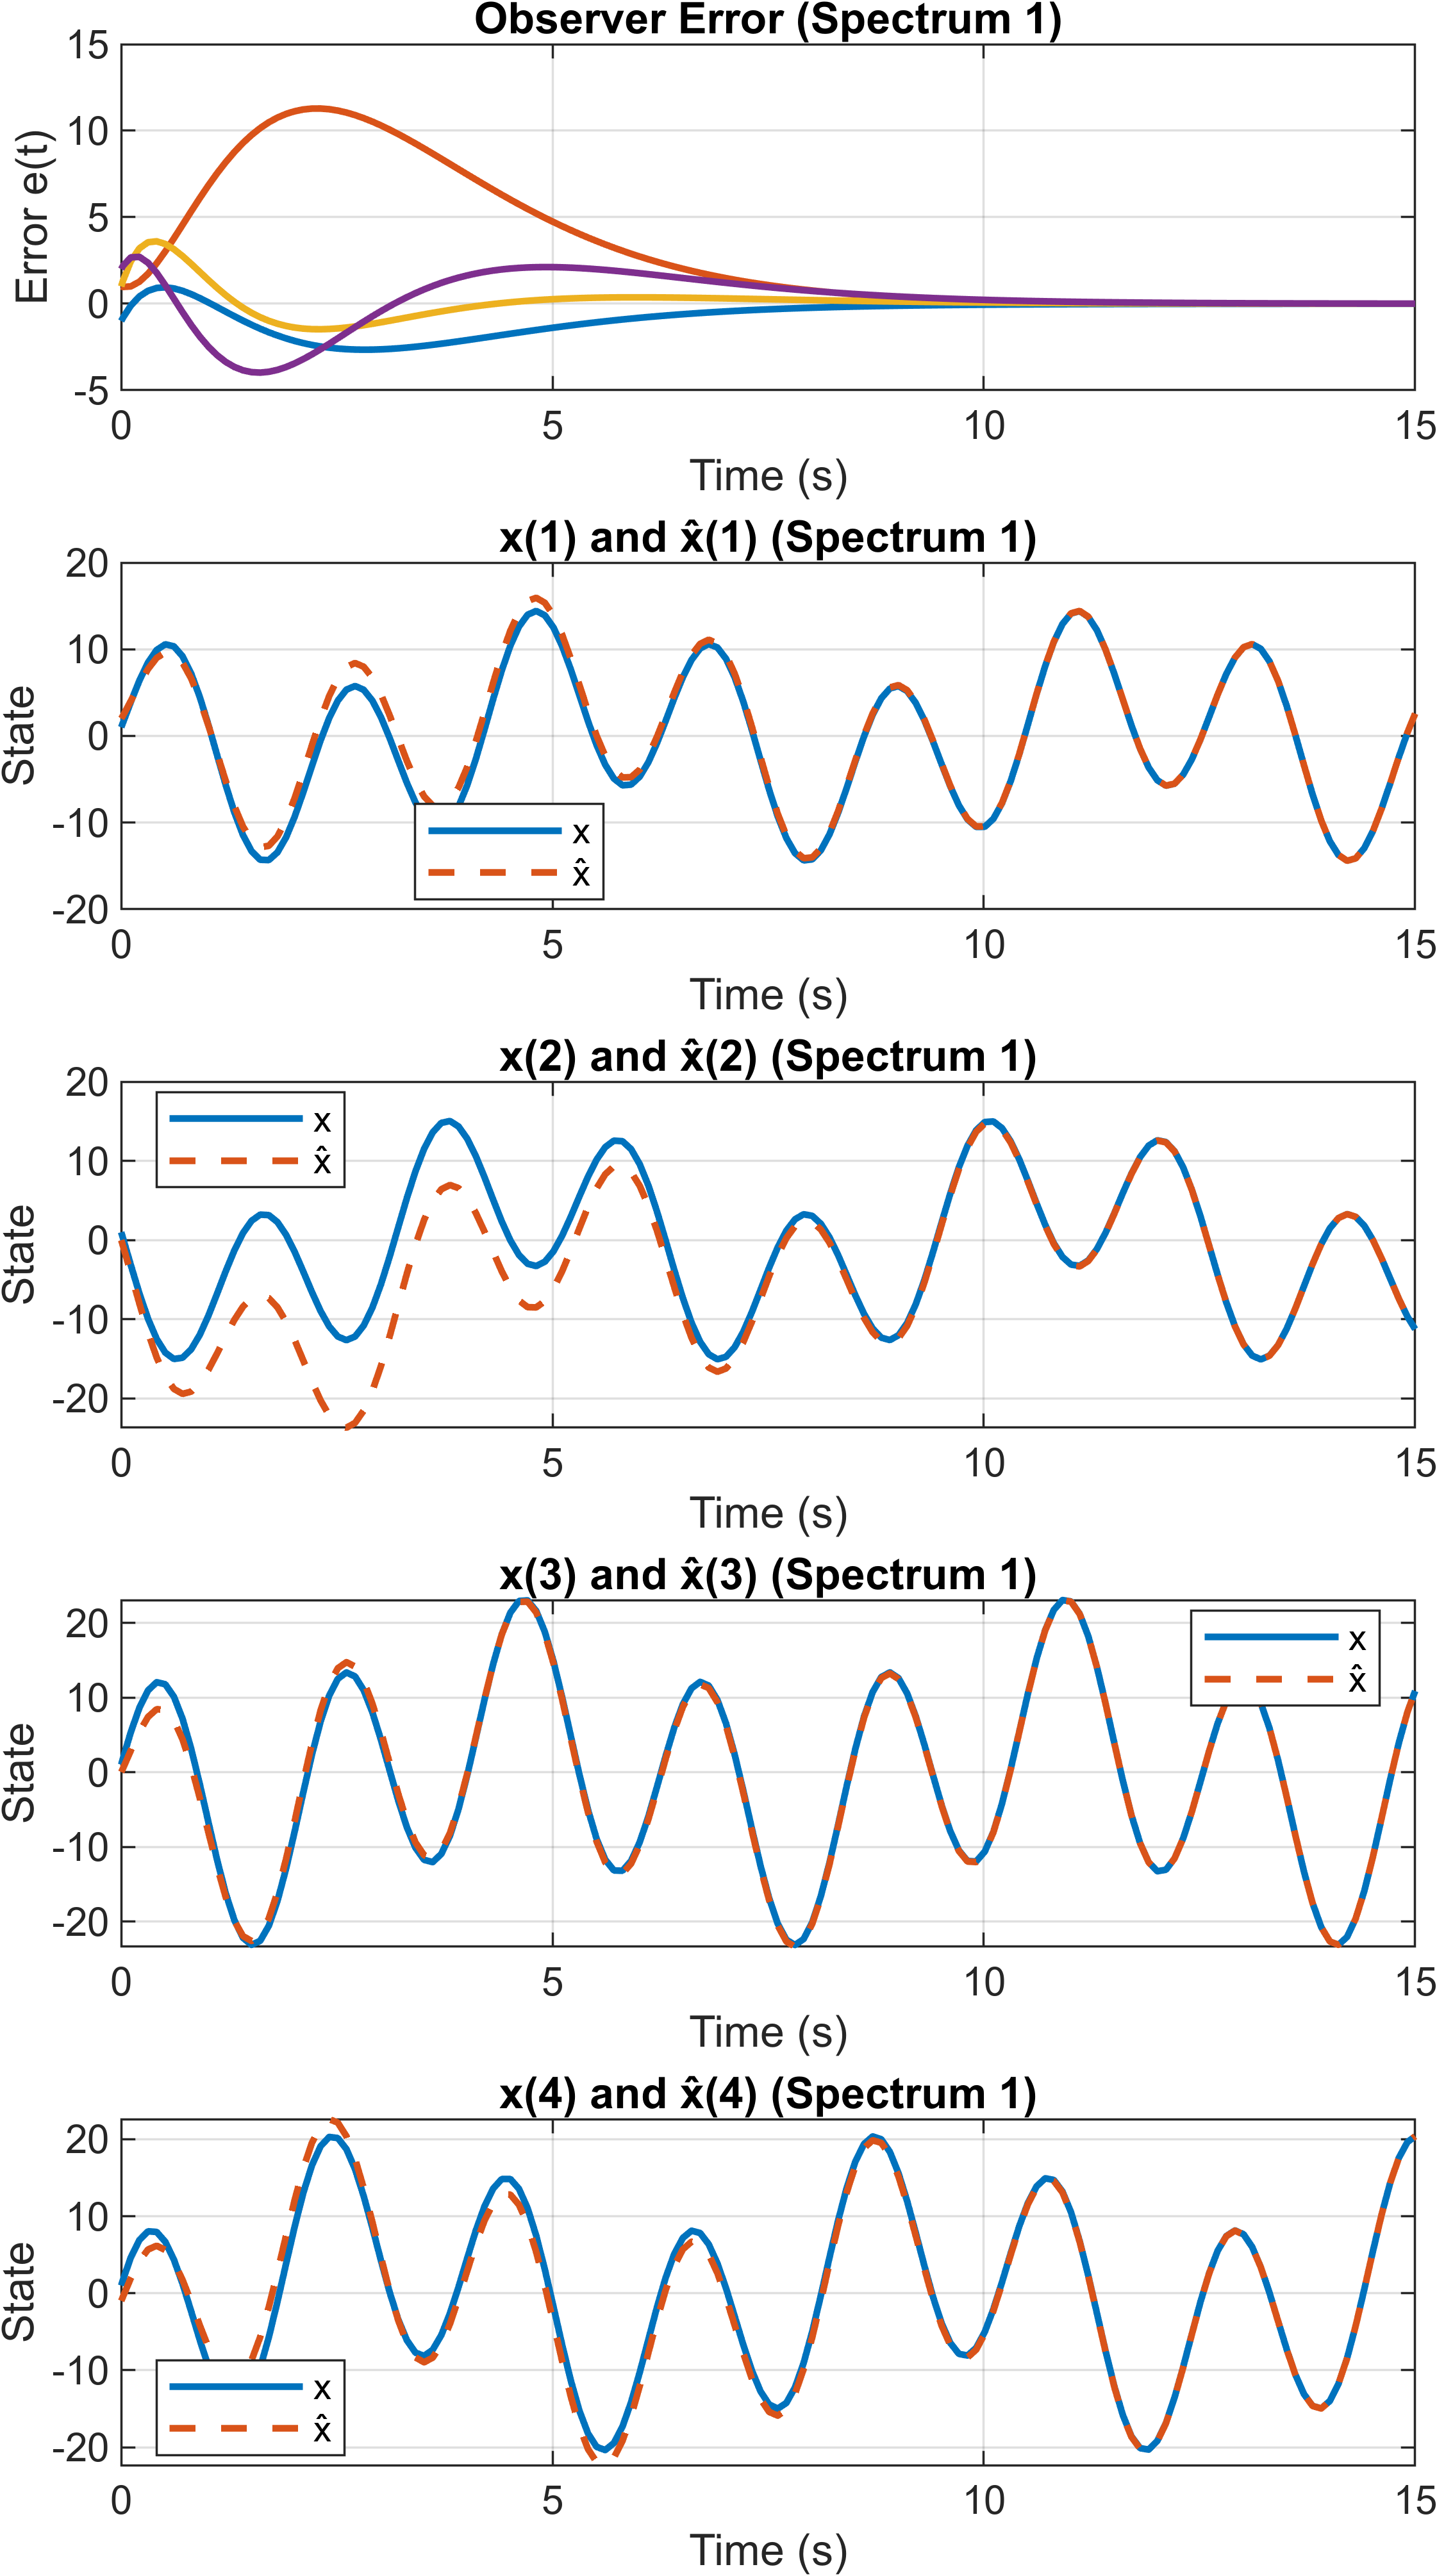
\includegraphics[width=0.8\linewidth]{figs/task2_1.png}
    \caption{Система с наблюдателем под первый спектр}
    \label{fig:2_1}
\end{figure}


\subsubsection{Второй спектр}

Теперь аналогично получим спектр $\{-1, -10, -100, -1000\}$.
Были выбраны такие матрицы
\begin{equation*}
    \Gamma=\begin{bmatrix}
        -1&  0&  0&  0\\
        0& -10&  0&  0\\
        0&  0& -100&  0\\
        0&  0&  0& -1000
    \end{bmatrix},\quad
    Y=\begin{bmatrix}
        1\\ 1\\ 1\\ 1
    \end{bmatrix}.
\end{equation*} 
С помощью CVX получаем
\begin{equation*}
    L=\begin{bmatrix}
        -739.7917\\
        -3.8772E+05\\
        2.5899E+04\\
        3.0300E+05
    \end{bmatrix}.
\end{equation*}
Проверим, что получен желаемый спектр
\begin{equation*}
    \sigma(A+LC)=\{-1000,\ -100,\ -10,\ -1\}.
\end{equation*}
Желаемый спектр успешно получен.
Выполним моделирование с начальными условиями системы 
$x(0) = \begin{bmatrix}
    1 & 1 & 1 & 1
\end{bmatrix}^T$ и наблюдателя $\hat x(0) = \begin{bmatrix}
    2 & 0 & 0 & -1
\end{bmatrix}^T$. Cравнительные графики $x(t)$ и $\hat x(t)$, 
а также график ошибки наблюдателя $e(t) = x(t) -\hat x(t)$
можно увидеть на \autoref{fig:2_2}.


\subsubsection{Третий спектр}

Аналогично получим спектр $\{-1 \pm 2i, -1 \pm 3i\}$.
Были выбраны такие матрицы
\begin{equation*}
    \Gamma=\begin{bmatrix}
        -1&  -2&  0&  0\\
        2& -1&  0&  0\\
        0&  0& -1&  -3\\
        0&  0&  3& -1
    \end{bmatrix},\quad
    Y=\begin{bmatrix}
        0\\ 1\\ 0\\ 1
    \end{bmatrix}.
\end{equation*} 
С помощью CVX получаем
\begin{equation*}
    L=\begin{bmatrix}
        -2.3333\\
        -8.1667\\
        -7.0833\\
        -2.2500
    \end{bmatrix}.
\end{equation*}
Проверим, что получен желаемый спектр
\begin{equation*}
    \sigma(A+LC)=\{
        -1.0000 + 3.0000i,\ 
        -1.0000 - 3.0000i,\ 
        -1.0000 + 2.0000i,\ 
        -1.0000 - 2.0000i
        \}.
\end{equation*}
Желаемый спектр успешно получен.
Выполним моделирование с начальными условиями системы 
$x(0) = \begin{bmatrix}
    1 & 1 & 1 & 1
\end{bmatrix}^T$ и наблюдателя $\hat x(0) = \begin{bmatrix}
    2 & 0 & 0 & -1
\end{bmatrix}^T$. Cравнительные графики $x(t)$ и $\hat x(t)$, 
а также график ошибки наблюдателя $e(t) = x(t) -\hat x(t)$
можно увидеть на \autoref{fig:2_3}.


\begin{figure}[H]
    \centering
    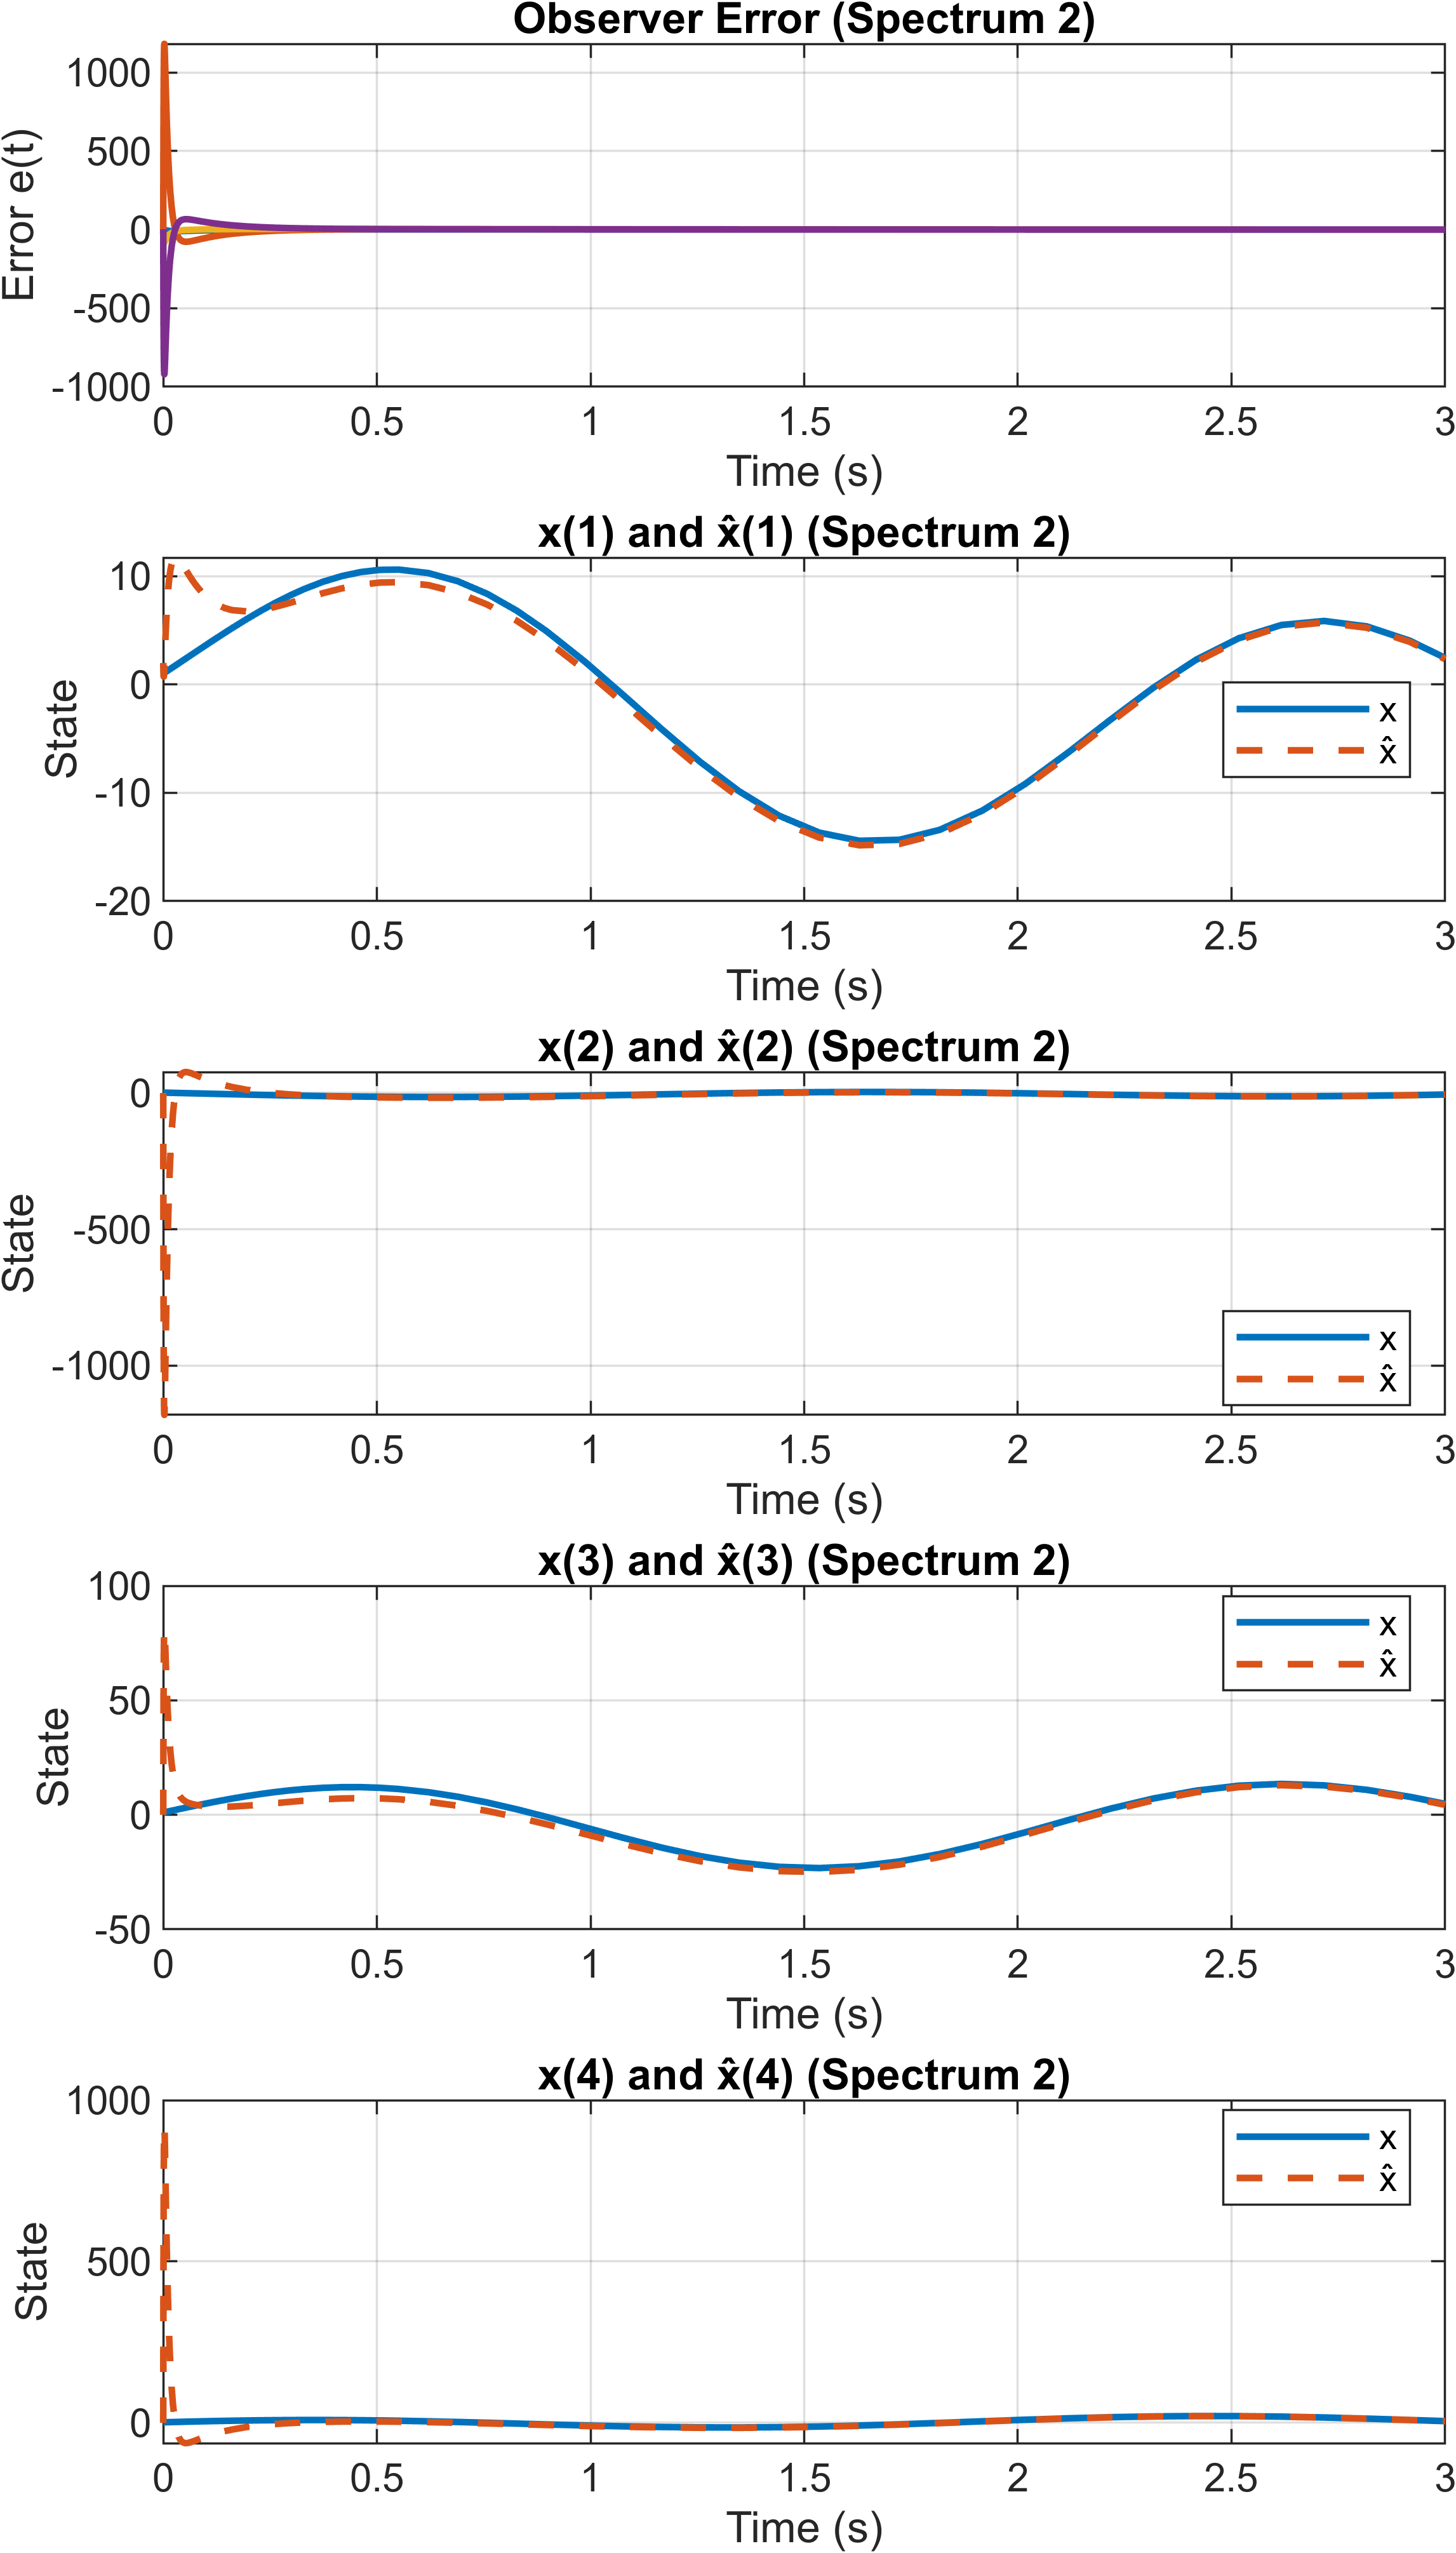
\includegraphics[width=0.8\linewidth]{figs/task2_2.png}
    \caption{Система с наблюдателем под второй спектр}
    \label{fig:2_2}
\end{figure}


\begin{figure}[H]
    \centering
    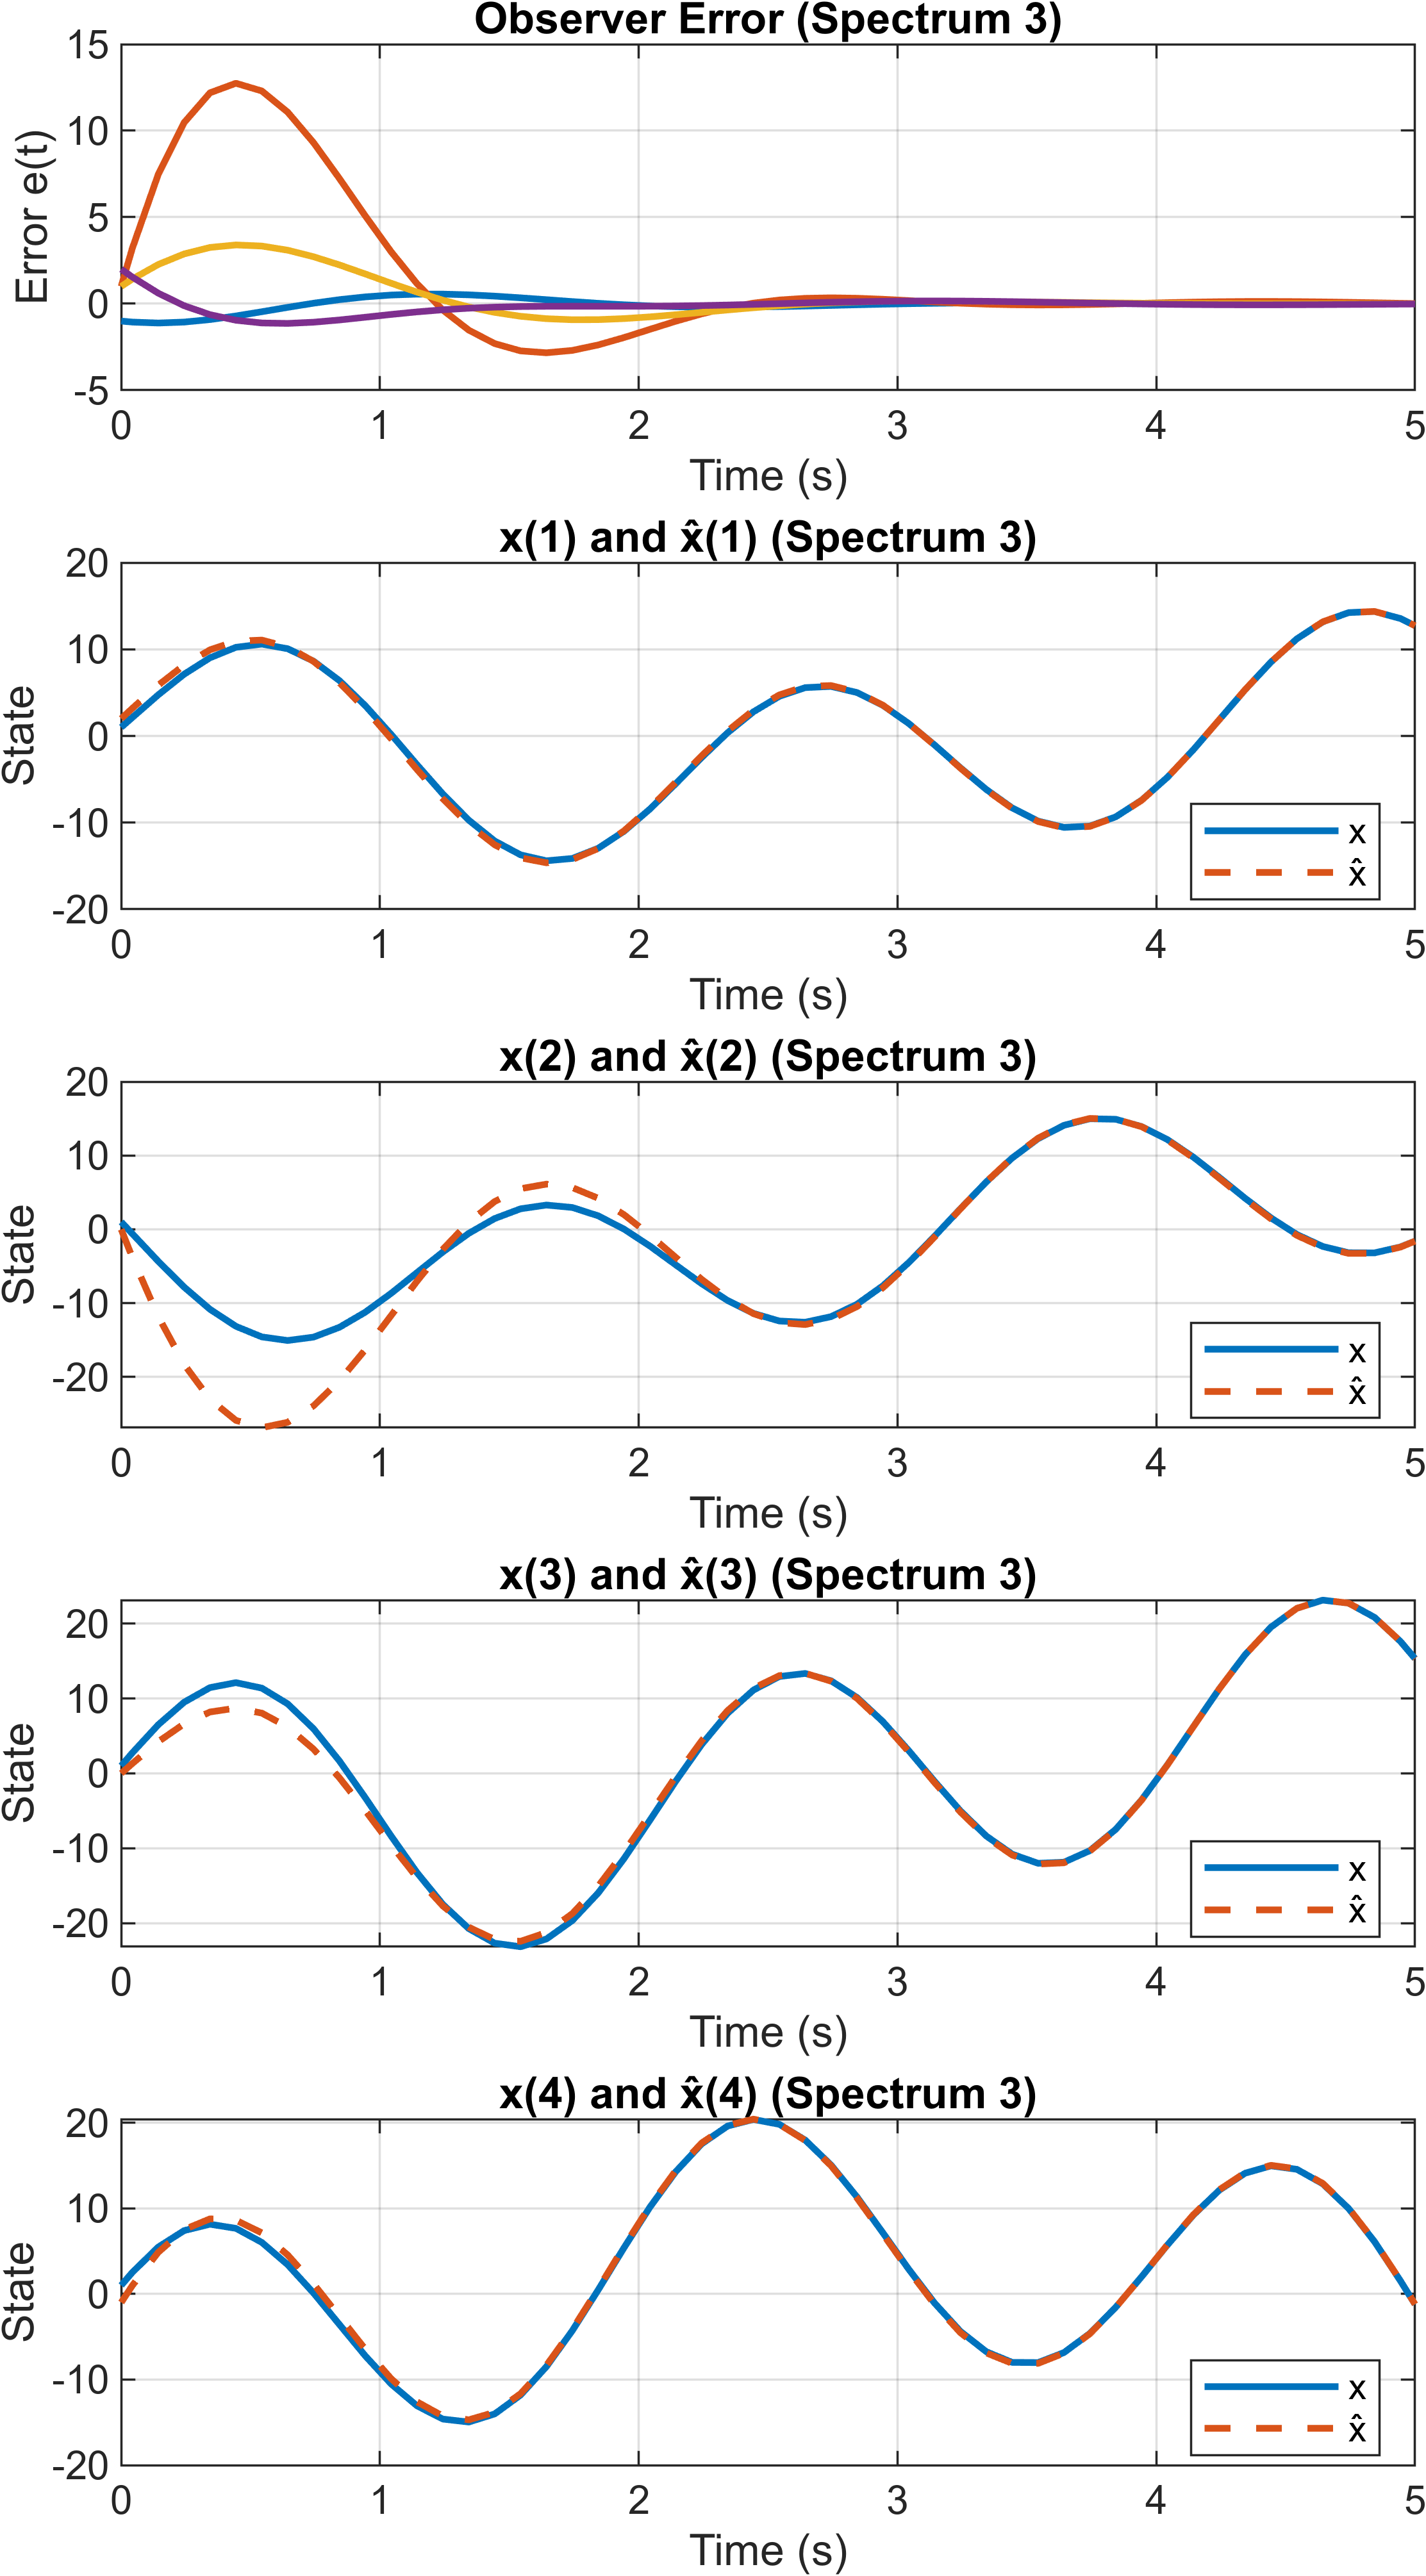
\includegraphics[width=0.8\linewidth]{figs/task2_3.png}
    \caption{Система с наблюдателем под третий спектр}
    \label{fig:2_3}
\end{figure}


\subsection{Вывод}

Сопоставим результаты компьютерного моделирования для рассмотренных спектров.
Для первого спектра $\{-1, -1, -1, -1\}$:
\begin{itemize}
    \item Наблюдатель сходится к состоянию системы примерно за 13 секунд.
    \item Ошибка наблюдателя $e(t)$ плавно стремится к нулю.
\end{itemize}
Для второго спектра $\{-1, -10, -100, -1000\}$:
\begin{itemize}
    \item Наблюдатель сходится к состоянию системы примерно за 3 секунды.
    \item Ошибка наблюдателя $e(t)$ очень быстро стремится к нулю с ОГРОМНЫМ
    перерегулированием.
    \item Требуются очень большие значения коэффициентов матрицы $L$, 
    что может быть непрактично в реальных системах.
\end{itemize}
Для третьего спектра $\{-1 \pm 2i, -1 \pm 3i\}$:
\begin{itemize}
    \item Наблюдатель сходится к состоянию системы примерно за 4 секунды.
    \item Ошибка наблюдателя $e(t)$ демонстрирует колебательное поведение 
    перед стабилизацией.
\end{itemize}
Сравнительные преимущества и недостатки:
\begin{itemize}
    \item Первый спектр обеспечивает плавную до относительнл долгую сходимость наблюдателя, 
    что делает его подходящим для систем, где требуется плавность.
    \item Второй спектр обеспечивает самую быструю сходимость наблюдателя, 
    но требует очень больших значений коэффициентов матрицы $L$.
    \item Третий спектр обеспечивает быструю сходимость наблюдателя,
    но с колебательным поведением, что может быть полезно в системах, 
    где допустимы колебания.
\end{itemize}



\section{Модальное управление по выходу}

Рассмотрим систему 
\begin{equation*}
    \begin{cases}
        
    \end{cases}
\end{equation*}